% cd ..\..\Users\NikitaSkybytskyi\Desktop\c3s1\complex-analysis
% cls && pdflatex lec-03.tex && pdflatex lec-03.tex && del lec-03.out, lec-03.log, lec-03.aux && start lec-03.pdf

% \documentclass[a4paper, 12pt]{article}
\usepackage[utf8]{inputenc}
\usepackage[english, ukrainian]{babel}

\usepackage{amsmath, amssymb}
\usepackage{multicol}
\usepackage{graphicx}
\usepackage{float}

\usepackage{amsthm}
\newtheorem{theorem}{Теорема}[subsection]
\newtheorem*{theorem*}{Теорема}
\newtheorem{lemma}{Лема}[subsection]
\newtheorem*{lemma*}{Лема}
\theoremstyle{definition}
\newtheorem*{remark*}{Зауваження}
\newtheorem*{example}{Приклад}

\newcommand{\Max}{\max\limits}
\newcommand{\Sum}{\sum\limits}
\newcommand{\Int}{\int\limits}
\newcommand{\Lim}{\lim\limits}

\newcommand{\RR}{\mathbb{R}}
\newcommand{\ZZ}{\mathbb{Z}}

\newcommand*\diff{\mathop{}\!\mathrm{d}}
\newcommand*\Diff[1]{\mathop{}\!\mathrm{d^#1}}

\DeclareMathOperator{\Real}{Re}
\DeclareMathOperator{\Imag}{Im}

\DeclareMathOperator{\Ln}{Ln}

\DeclareMathOperator{\Arg}{Arg}

\DeclareMathOperator{\Arctan}{Arctan}
\DeclareMathOperator{\Arcsin}{Arcsin}
\DeclareMathOperator{\Arccos}{Arccos}
\DeclareMathOperator{\Arccosh}{Arccosh}
\DeclareMathOperator{\Arctanh}{Arctanh}

\DeclareMathOperator{\arcsinh}{arcsinh}
\DeclareMathOperator{\arccosh}{arccosh}
\DeclareMathOperator{\arctanh}{arctanh}
\DeclareMathOperator{\arccoth}{arccoth}

\newcommand{\varLimsup}{\varlimsup\limits}

\renewcommand{\epsilon}{\varepsilon}
\renewcommand{\phi}{\varphi}

\allowdisplaybreaks
\setlength\parindent{0pt}

\usepackage{xcolor}
\usepackage{hyperref}
\hypersetup{unicode=true,colorlinks=true,linktoc=all,linkcolor=red}

\numberwithin{equation}{section}% reset equation counter for sections
\numberwithin{equation}{subsection}
% Omit `.0` in equation numbers for non-existent subsections.
\renewcommand*{\theequation}{%
  \ifnum\value{subsection}=0 %
    \thesection
  \else
    \thesubsection
  \fi
  .\arabic{equation}%
}


% \begin{document}

\setcounter{section}{2}
\section{Елементарні функції}

Цей параграф присвячений елементарним функціям комплексної змінної та їхнім геометричним ілюстраціям -- відображенням, які вони здійснюють. Ці функції є природнім розповсюдженням функцій дійсної змінної у комплексну площину. \\

Одначе, при такому розповсюдженні функції інколи набувають нових, дивних властивостей. Так, функція $e^z$ виявляється періодичною, а $\sin z$ і $\cos z$ -- необмеженими. Ба більше, вдається визначити логарифм від'ємних (і взагалі довільних нерівних нулеві комплексних чисел). \\

В другому пункті ми особливо виділяємо просту дробово-раціональну функцію $w = \frac12 \left(z + \frac 1z\right)$ у зв'язку з її важливістю для практичних задач.

\subsection{Функції $w = z^n$ і $w = \sqrt[n]{z}$}

Вже визначені в розділі 1 для всіх комплексних $z$. Перша з цих функцій
\begin{equation}
	\label{eq:3.1.1}
	w = z^n
\end{equation}
однозначна. \\

Якщо в площинах $z$ і $w$ ввести полярні координати 
\begin{equation}
	\label{eq:3.1.2}
	z = r (\cos \phi + i \sin \phi),\quad w = \rho (\cos \theta + i \sin \theta),
\end{equation}
то співвідношення \eqref{eq:3.1.1} можна представити у вигляді двох рівностей
\begin{equation}
	\label{eq:3.1.3}
	\rho = r^n, \quad \theta = n \phi,
\end{equation}
які пов'язують дійсні величини. \\

З \eqref{eq:3.1.3} видно, що відображення, яке здійснює функція $w = z^N$ зводиться до повороту кожного вектора $z \ne 0$ на кут $(n - 1) \arg z$ і розтягнення його у $|z|^{n-1}$ разів. \\

Далі зрозуміло, що точки $z_1$ і $z_2$ з рівними модулями та аргументами які відрізняються на кратне $2 \pi / n$ переходять при відображенні \eqref{eq:3.1.1} в одну точку. \\

Як наслідок, для однолистості відображення $w = z^n$ у деякій області $D$ необхідно і достатньо, аби $D$ не містила жодних двох точок $z_1$ і $z_2$ пов'язаних співвідношеннями
\begin{equation}
	\label{eq:3.1.4}
	|z_1| = |z_2|; \quad \arg z_1 = \arg z_2 + \dfrac{2 k \pi}{n} \quad (k \in \ZZ, k \ne 0).
\end{equation}

Цій умові задовольняють, наприклад, сектори
\begin{equation}
	\label{eq:3.1.5}
	\frac{2\pi k}{n} < \phi < \frac{2\pi(k+1)}{n}, \quad (k = 0, 1, 2, \ldots),
\end{equation}
кожен з яких при відображенні \eqref{eq:3.1.1} перетворюється у площину $w$ з виключеною додатною піввіссю.  \\

При цьому промені з вершиною у точці $z = 0$ переходять у промені з вершиною у точці $w$ (тобто лише повертаються на деякий кут); дуги кіл з центром $z = 0$ -- у дуги кіл з центром $w$ (тільки, взагалі кажучи, іншого радіуса). На наступому малюнку зображений прообраз в одному з таких секторів площини $z$ сітки полярних і декартових координат у площині $w$ відповідно:

\begin{figure}[H]
	\centering
	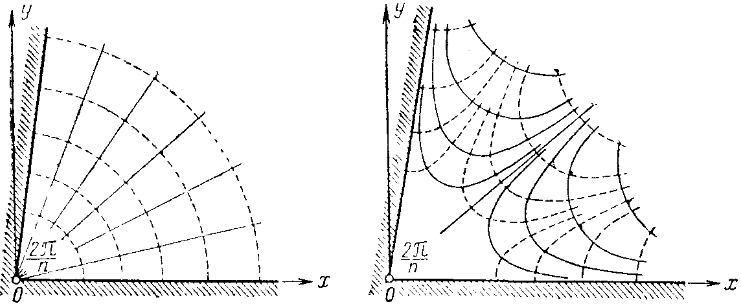
\includegraphics[width=.8\linewidth]{mal-09.png}
\end{figure}

Справді, з рівносильної до \eqref{eq:3.1.1} формули
\begin{equation}
	\label{eq:3.1.6}
	w = u + i v = r^n \cdot (\cos n \phi + i \sin \phi)
\end{equation}
випливає, що прямим $u = u_0$ і $v = v_0$ у площині $z$ відповідають криві з полярними рівнянням
\begin{equation}
	\label{eq:3.1.7}
	r = \sqrt[n]{\frac{u_0}{\cos n\phi}}; \quad r = \sqrt[n]{\frac{v_0}{\sin n\phi}}.
\end{equation}

Зауважимо нарешті, що функція $w = z^n$ аналітична у всій площині, адже для довільного $z$ існує
\begin{equation}
	\label{eq:3.1.8}
	\Lim_{h \to 0} \left(\dfrac{(z + h)^n - z^n}{h}\right) = \Lim_{h \to 0} \left(\dfrac{n \cdot z^{n - 1} \cdot h + h^2 \cdot (\cdots)}{h}\right) = n \cdot z^{n - 1}.
\end{equation}

Функція
\begin{equation}
	\label{eq:3.1.9}
	w = \sqrt[n]{z},
\end{equation}
обернена до функції $z = w^n$, $n$-значна при $z \ne 0$. Як випливає з розділу 2, значення кореня $\sqrt[n]{z}$ визначається значенням аргументу, вибраним для точки $z$. \\

Позначимо через $\arg z_0$ одне зі значень аргументу в точці $z_0 \ne 0$ і припустимо, що точка $z$ описує, починаючи з $z_0$, деяку неперервну лінію $C$, яка не проходить через початок координат. \\

Через $\arg z$ ми будемо позначати те значення аргументу, яке змінюється при цьому неперервно. \\

В силу неперервності $\arg z$ і $|z|$ значення $w = \sqrt[n]{z}$, яке цілком визначається зробленим вибором аргументу також буде змінюватися неперервно. \\

Припустимо, що крива $C$ замкнута і не містить всередині себе точку $z = 0$. \\

Тоді, при повному обході точкою $z$ кривої $C$, точка $w = \sqrt[n]{z}$, де $\sqrt[n]{z}$ -- вибране нами значення кореня, описує деяку замкнуту криву $\Gamma$, повертаючись до свого початкового положення, бо при цьому $\arg z$ повертається до початкового значення $\arg z_0$. \\

Значення кореня, які визначаються іншим вибором початкового значення $\arg z_0$ при повному обході $C$ також описують замкнуті криві $\Gamma_k$, які відрізняються від кривої $\Gamma$ тільки поворотами на ціле кратне кута $2 \pi / n$:
\begin{figure}[H]
	\centering
	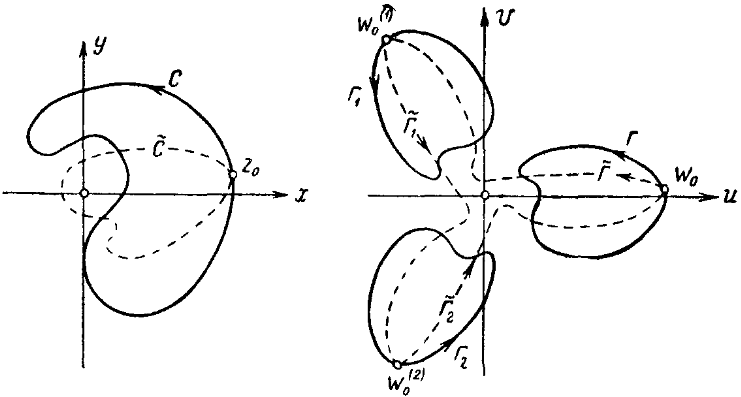
\includegraphics[width=.8\linewidth]{mal-10.png}
	% \caption{дія функції $w = \sqrt[n]{z}$ на різні криві}
\end{figure}

Нехай тепер $\tilde{C}$ -- замкнута крива без точок самоперетину, яка містить точку $z = 0$ всередині себе, і $z_0$ -- деяка точка кривої $\tilde{C}$. \\

Тоді, при повному обході $\tilde{C}$, починаючи з $z_0$ у додатному напрямку, відповідна точка $w = \sqrt[n]{z}$ не повертається у своє початкове положення, а займає нове положення
\begin{equation}
	\label{eq:3.1.10}
	w_0^{(1)} = \left(\cos \left( \dfrac{2 \pi}{n} \right) + i \sin \left( \dfrac{2 \pi}{n} \right) \right) w_0
\end{equation} -- значення $\sqrt[n]{z_0}$ відмінне від $w_0$. \\

Це пояснюється тим, що $\arg z$ при обході кривої $\tilde{C}$ збільшується на $2 \pi$. \\

Звідси випливає, що у довільній області $D$ яка не містить жодної замкнутої кривої, що обходить точку $z = 0$ можна виділити $n$ неперервних і однозначних функцій, кожна з яких набуває одного зі значень $\sqrt[n]{z}$. \\

Ці $n$ функцій називаються гілками багатозначної функції $w = \sqrt[n]{z}$, їх значення в кожній фіксованій точці відрізняються один від одного множником
\begin{equation}
	\label{eq:3.1.11}
	\cos \left( \dfrac{2 k \pi}{n} \right) + i \sin \left( \dfrac{2 k \pi}{n} \right).
\end{equation}

Кожна така гілка буде реалізувати однолисте відображення області $D$, тому в кожній точці цієї області застосовна теорема про прохідну оберненої функції (п. 5), згідно з якою існує цілком конкретне значення похідної
\begin{equation}
	\label{eq:3.1.12}
	\left( \sqrt[n]{z} \right)^\prime = \dfrac{1}{(w^n)'} = \dfrac{1}{n} \cdot \dfrac{\sqrt[n]{z}}{z},
\end{equation}
або, якщо домовимося писати $\sqrt[n]{z} = z^{1 / n}$,
\begin{equation}
	\label{eq:3.1.13}
	\left( z^{1 / n} \right)^\prime = \dfrac{z^{1 / n - 1}}{n}.
\end{equation}

Таким чином, довільна із побудованих гілок є аналітичною функцією в області $D$. \\

В області $D$ розглядуваного типу і нескінченнозначна функція $\Arg z$ розпадається на нескінченну кількість неперервних і однозначних гілок. \\

Кожну таку гілку ми будемо позначати символом $\arg z$ і кожного разу будемо вказувати, яка ця гілка визначається. \\

Якщо область $D$ містить хоча б одну замкнуту криву, яка обходить точку $z = 0$, то у такій області гілки функції $\sqrt[n]{z}$ неможливо відділити одну від одної. \\

Якщо в околі деякої точки $z \ne 0$ з області $D$ ми і виділимо якусь гілку, то, рухаючись по кривій, яка обходить $z = 0$, ми прийдемо до іншої гілки. \\

Відповідно, в такій області $D$ ми не можемо розглядати функцію $\sqrt[n]{z}$ як сукупність окремих однозначних аналітичних функцій. \\

Точка $z = 0$, в довільному околі якої неможливо відділити $n$ окремих гілок функції $\sqrt[n]{z}$ називаються \textit{точкою гілкування} цієї функції. \\

У якості прикладу області $D$ першого типу можна розглядати площину $z$ з вирізаною лінією $L$ яка йде від точки $z = 0$ до нескінченності. \\

Якщо $L$ збігається з додатною піввіссю, то гілки функції $w = \sqrt[n]{z}$ відображає область $D$ на сектори
\begin{equation}
	\label{eq:3.1.14}
	\dfrac{2 k \pi}{n} < \arg w < \dfrac{2 (k + 1) \pi}{n}.
\end{equation}

Ці відображення обернені до розглянутого вище відображення за допомогою функції $w = z^n$. \\

Область $D$ напевне є областю другого типу якщо вона містить точку $z = 0$ всередині.

\subsection{Функція Жуковського $w = \frac{1}{2} \left( z + \frac{1}{z} \right)$}

Визначена, однозначна та аналітична для всіх $z \ne 0$. \\

Знайдемо область однолистості відображення
\begin{equation}
	\label{eq:3.2.1}
	w = \frac{1}{2} \left( z + \frac{1}{z} \right).
\end{equation}

Для цього припустимо, що $z_1 \ne z_2$ переходять в одну і ту ж точку $w$. \\

Тоді маємо
\begin{equation}
	\label{eq:3.2.2}
	z_1 + \frac{1}{z_1} = z_2 + \dfrac{1}{z_2},
\end{equation}
звідки
\begin{equation}
	\label{eq:3.2.3}
	(z_1 - z_2) \cdot \left( 1 - \dfrac{1}{z_1 \cdot z_2} \right) = 0
\end{equation}
і, як наслідок,
\begin{equation}
	\label{eq:3.2.4}
	z_1 \cdot z_2 = 1.
\end{equation}

Таким чином, для однолистості відображення \eqref{eq:3.2.1} у деякій області $D$ необхідно і достатньо, щоб $D$ не містила жодних двох точок $z_1$ і $z_2$, пов'язаних співвідношенням $z_1 \cdot z_2 = 1$. \\

Цій умові задовольняє, наприклад, внутрішність одиничного круга $|z| < 1$ або його зовнішність $|z| > 1$. \\

Для того, зоб вивчити картину відображення \eqref{eq:3.2.1}, покладемо 
\begin{equation}
	\label{eq:3.2.5}
	z = r \left( \cos \phi + i \sin \phi \right), \quad w = u + i v
\end{equation}
і виділимо дійсну та уявну частини. \\

Тоді відображення \eqref{eq:3.2.1} перепишеться у вигляді
\begin{equation}
	\label{eq:3.2.6}
	u = \dfrac 12 \left( r + \dfrac 1r \right) \cos \phi, \quad v = \dfrac 12 \left( r - \dfrac 1r \right) \sin \phi,
\end{equation}
і ми побачимо, що кожне коло $|z| = r_0 < 1$ переходить з його допомогою у криву
\begin{equation}
	\label{eq:3.2.7}
	u = \dfrac 12 \left( r_0 + \dfrac{1}{r_0} \right) \cos \phi, \quad v = - \dfrac 12 \left( \dfrac{1}{r_0} - r_0 \right) \sin \phi,
\end{equation}
тобто в еліпс з півосями 
\begin{equation}
	\label{eq:3.2.8}
	a = \dfrac 12 \left( r_0 + \dfrac{1}{r_0} \right), \quad b = \dfrac 12 \left( \dfrac{1}{r_0} - r_0 \right),
\end{equation}
який проходиться у від'ємному напрямку. \\

При $r_0 \to 1$ цей еліпс стискається у відрізок $[-1, 1]$ осі $u$, а при $r_0 \to 0$ розходиться на нескінченність. \\

Відповідно, функція \eqref{eq:3.2.1} відображає внутрішність круга $|z| < 1$ на зовнішність відрізка $[-1, +1]$:
\begin{figure}[H]
	\centering
	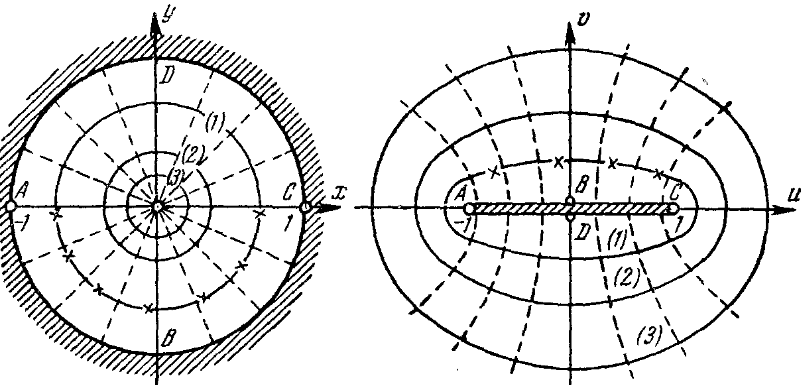
\includegraphics[width=.8\linewidth]{mal-11.png}
	%\caption{дія функції Жуковського}
\end{figure}

Всі внутрішні точки цього відрізка -- подвійні, він немовби складається із двох берегів, причому верхнє півколо переходить у нижній берег, а нижнє півколо у верхній берег. \\

Помітимо ще, що радіуси $\arg z = \phi_0$, $0 < r < 1$ переходять при відображенні \eqref{eq:3.2.1} у гілки гіпербол
\begin{equation}
	\label{eq:3.2.9}
	\dfrac{u^2}{\cos^2 \phi_0} - \dfrac{v^2}{\sin^2 \phi_0} = 1
\end{equation}

Фокуси цих гіпербол, так само як і еліпсів \eqref{eq:3.2.7} розташовані у кінцях відрізка $[-1, +1]$. \\

Зі співвідношень \eqref{eq:3.2.6} випливає також, що кола $|z| = r_0 > 1$ переходять в еліпси із півосями
\begin{equation}
	\label{eq:3.2.10}
	a = \dfrac 12 \left( r_0 + \dfrac{1}{r_0} \right), \quad b = \dfrac 12 \left( r_0 - \dfrac{1}{r_0} \right)
\end{equation}

Ці еліпси збігаються з тими, у які переходять кола $|z| = r_0 < 1$, тільки обходяться вони у додатному напрямку. \\

Відповідно, функція \eqref{eq:3.2.1} відображає і зовнішність круга $|z| > 1$ також на зовнішність відрізка $[-1, +1]$ осі $u$, причому верхнє півколо переходить у верхній берег відрізка, а нижня -- в нижній. \\

Обернена до функції \eqref{eq:3.2.1} функція
\begin{equation}
	\label{eq:3.2.11}
	z = w + \sqrt{w^2 - 1}
\end{equation}
двозначна -- кожній точці $w$ вона ставить у відповідність дві точки $z_1$ і $z_2$, пов'язані умовою $z_1 \cdot z_2 = 1$. \\

Якщо покласти $z_1 = w + \sqrt{w^2 - 1}$, то другим значенням $z$, яке відповідає $w$ буде $z_2 = w - \sqrt{w^2 - 1}$ і безпосередньо видно, що $z_1 \cdot z_2 = 1$. \\

Позначимо через $\rho_1$, $\theta_1$ і $\rho_2$, $\theta_2$ модулі і аргументи комплексних чисел $w - 1$ і $w + 1$ відповідно. \\

Тоді модуль і аргумент кореня у формулі \eqref{eq:3.2.11} будуть дорівнювати $\sqrt{\rho_1 \cdot \rho_2}$ і $(\theta_1 + \theta_2) / 2$. \\

Звідси випливає, що при обході точкою $w$ замкнутої лінії першого або другого типу, який охоплює лише одну із точок $+1$ і $-1$, значення кореня змінює знак. \\

Справді, при такому обході $\theta_1$ (або $\theta_2$) змінюється на $2 \pi$, а $\theta_2$ (або $\theta_1$) не змінюється. \\

Відповідно, аргумент кореня змінюється на $\pi$, а модуль кореня при обході довільного замкнутого контуру повертається до початкового значення. \\

Якщо тепер точка $w$ обходить замкнуту лінію третього типу яка охоплює обидві точки $\pm1$, то значення кореня не змінюється, бо при цьому і $\theta_1$ і $\theta_2$ змінюються на $2 \pi$ і, відповідно, аргумент кореня $(\theta_1 + \theta_2) / 2$ також змінюється на $2 \pi$.
\begin{figure}[H]
	\centering
	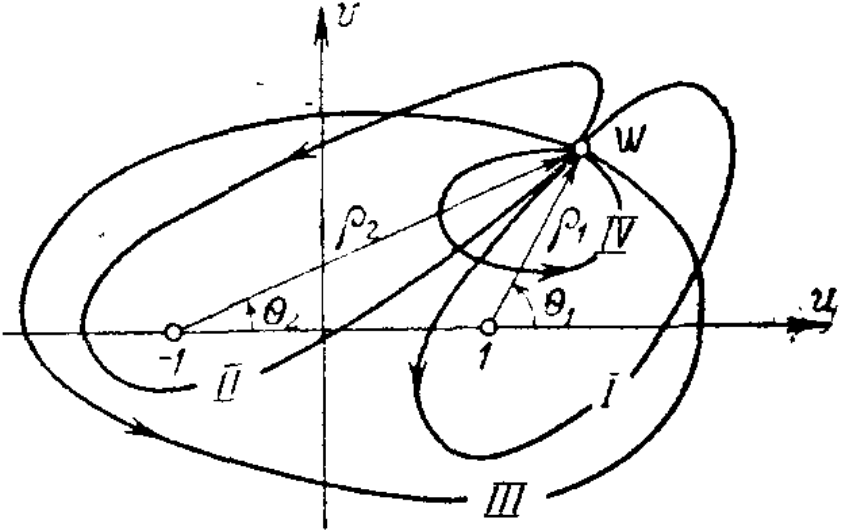
\includegraphics[width=.6\linewidth]{mal-12.png}
	%\caption{дія функції $z = w + \sqrt{w^2 - 1}$ при обході різних типів кривих}
\end{figure}

Значення кореня не змінюється якщо замкнута лінія має четвертий тип, тобто не містить всередині себе жодної з точок $\pm 1$, адже при цьому ані $\theta_1$ ані $\theta_2$ не змінюються. \\

Таким чином, в довільній області $\Delta$ у якій не можна провести замкнуту лінію яка обходить тільки одну з точок $\pm 1$ функція \eqref{eq:3.2.11} допускає виділення двох однозначних гілок. \\

Ці гілки у кожній фіксованій точці $w$ відрізняються знаком кореня у формулі \eqref{eq:3.2.11} і призводять до двох значень $z$ зв'язаних умовою $z_1 \cdot z_2 = 1$. \\

Кожна з цих гілок реалізує однолисте відображення і, за теоремою про похідну оберненої функції, аналітична. \\

Якщо ж в області $\Delta$ можна обійти точку $+1$ (не обійшовши при цьому точку $-1$) або $-1$ (не обійшовши $+1$), наприклад, якщо $\Delta$ містить всередині хоча б одну з цих точок, то у такій області гілки функції \eqref{eq:3.2.11} неможливо відрізнити одну від одної. \\

Точки $w = \pm 1$, у яких гілки функції \eqref{eq:3.2.11} немовби з'єднуються між собою, називаються точками гілкування цієї функції. \\

У якості прикладу області $\Delta$ першого типу можна розглянути площину $w$ із вирізаною лінією $\Lambda$ яка з'єднує точки $-1$ і $+1$. \\

Якщо ж $\Lambda$ є відрізком $[-1,+1]$ дійсної вісі, то дві гілки функції \eqref{eq:3.2.11} відображають $\Delta$, відповідно на зовнішність та внутрішність одиничного кола. \\

Ці відображення обернені до розглянутих вище.

\subsection{Експонента і логарифм}

Експоненту $e^z$ визначимо для довільного комплексного $z = x + i y$ наступною рівністю:
\begin{equation}
	\label{eq:3.3.1}
	w = e^z = e^{x + i y} = e^x (\cos y + i \sin y).
\end{equation}

Для дійсних $z = x$ це визначення збігається зі звичайним. \\

Експонента всюди аналітична. Справді, у довільній точці виконуються умови Коші-Рімана:
\begin{align}
	\label{eq:3.3.2}
	\dfrac{\partial}{\partial x} (e^x \cos y) &= \dfrac{\partial}{\partial y} (e^x \sin y); \\
	\label{eq:3.3.3}
	\dfrac{\partial}{\partial y} (e^x \cos y) &= - \dfrac{\partial}{\partial x} (e^x \sin y).
\end{align}

Зберігається звичайна формула диференціювання
\begin{equation}
	\label{eq:3.3.4}
	(e^z)' = e^z.
\end{equation}
Справді, похідна не залежить від напрямку, тому маємо
\begin{equation}
	\label{eq:3.3.5}
	(e^z)' = \dfrac{\partial}{\partial x} (e^x (\cos y + i \sin y)) = e^x (\cos y + i \sin y) = e^z.
\end{equation}

Зберігається основна властивість експоненти:
\begin{multline}
	\label{eq:3.3.6}
	e^{z_1} \cdot e^{z_2} = e^{x_1} \cdot (\cos y_1 + i \sin y_1) \cdot e^{x_2} \cdot (\cos y_2 + i \sin y_2) = \\
	= e^{x_1 + x_2} \cdot (\cos(y_1 + y_2) + i \cdot \sin(y_1+y_2)) = e^{z_1 + z_2}.
\end{multline}

Зауважимо, що експонента жодного комплексного числа не дорівнює нулю адже $|e^z| = e^x > 0$. \\

Покладаючи в \eqref{eq:3.3.1} $x = 0$, $y = \phi$ отримаємо класичну формулу Ейлера:
\begin{equation}
	\label{eq:3.3.7}
	e^{i \phi} = \cos \phi + i \sin \phi.
\end{equation}

За допомогою формули Ейлера довільне комплексне число $z$ з модулем $r$ і аргументом $\phi$ може бути записане у степеневій формі:
\begin{equation}
	\label{eq:3.3.8}
	z = r \cdot (\cos \phi + i \sin \phi) = r \cdot e^{i \phi}.
\end{equation}

Експонента періодична з чисто уявним періодом $2 \pi i$. Справді, для довільного цілого $k$ маємо
\begin{equation}
	\label{eq:3.3.9}
	e^{z + 2 \pi k i} = e^z \cdot e^{2 \pi k i} = e^z,
\end{equation}
адже, згідно з формулою Ейлера, $e^{2 \pi k i} = 1$. \\

Проте, якщо $e^{z_1} = e^{z_2}$, то $e^{x_1} = e^{x_2}$, $\cos y_1 = \cos y_2$, $\sin y_1 = \sin y_2$, тому $x_2 = x_1$, $y_2 = y_1 + 2 k \pi$, або
\begin{equation}
	\label{eq:3.3.10}
	z_2 - z_1 = 2 k \pi i,
\end{equation}
де $k$ -- ціле число. \\

Завдяки періодичності, вивчення функції $e^z$ на площині зводиться до вивчення її на смузі $0 \le y < 2 \pi$. \\

Зокрема, відображення \eqref{eq:3.3.10} однолисте на цій смузі, адже ця смуга не містить жодних двох точок, пов'язаних співвідношенням $e^{z_1} = e^{z_2}$. \\

Введемо у площині $w$ полярні координати, поклавши $w = \rho \cdot e^{i \theta}$, тоді \eqref{eq:3.3.1} запишеться у вигляді двох рівностей:
\begin{equation}
	\label{eq:3.3.11}
	\rho = e^x, \quad \theta = y.
\end{equation}

Як наслідок, відображення \eqref{eq:3.3.1} перетворює прямі $y = y_0$ у промені $\theta = y_0$, а відрізки $x = x_0$, $0 \le y < 2 \pi$ -- в кола $\rho = e^{x_0}$. \\

При цьому смуга $0 < y < 2 \pi$ перетворюється у площину $w$ із розрізом вздовж додатної півосі, а половина $0 < y < \pi$ цієї смуги -- у верхню півплощину. \\

У загальному випадку, смуга $0 < \Imag z < h$ експонента переводить в кути $0 < \arg w < h$:
\begin{figure}[H]
	\centering
	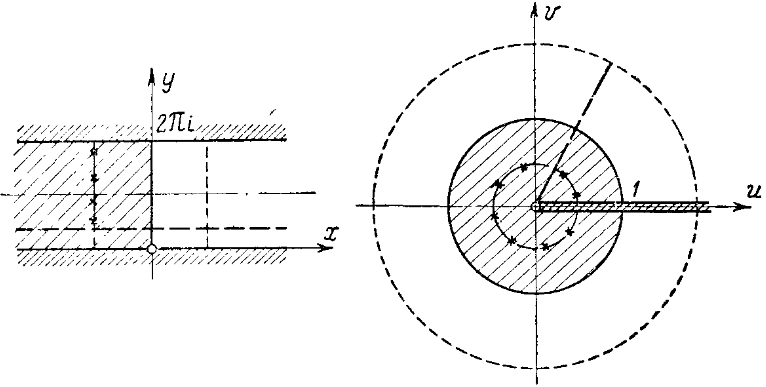
\includegraphics[width=.8\linewidth]{mal-13.png}
	%\caption{дія експоненти на різні області}
\end{figure}

Логарифм визначається як \textit{обернена} до експоненти функція: число $w$ називається логарифмом числа $z$ якщо $e^w = z$, позначається
\begin{equation}
	\label{eq:3.3.12}
	w = \ln z.
\end{equation}

З визначення випливає \textit{основна властивість логарифмів}: якщо $w_1 = \ln z_1$ і $w_2 = \ln z_2$, то $w = w_1 + w_2$ є логарифмом числа $z = z_1 \cdot z_2$:
\begin{equation}
	\label{eq:3.3.13}
	\ln z_1 + \ln z_2 = \ln (z_1 \cdot z_2).
\end{equation}

Справді, $z_1 = e^{w_1}$, $z_2 = e^{w_2}$, тому $z_1 \cdot z_2 = e^{w_1 + w_2}$. \\

Зокрема, покладаючи в \eqref{eq:3.3.13} $z_1 = |z|$, $z_2 = e^{i \arg z}$, отримаємо
\begin{equation}
	\label{eq:3.3.14}
	\ln z = \ln |z| + i \arg z,
\end{equation}
де символ $\arg z$ позначає \textit{довільне} значення аргументу $z$, тому кожне комплексне число $z \ne 0$ має нескінченну кількість логарифмів. \\

Для ясності будемо позначати \textit{багатозначну} функцію символом $\Ln z$:
\begin{equation}
	\label{eq:3.3.15}
	\Ln z = \ln |z| + i \Arg z = \ln r + i (\phi + 2 k \pi).
\end{equation}

Символом $\ln z$ будемо позначати \textit{одне} зі значень $\Ln z$, вказуючи за потреби яке саме. \\

Як і раніше, значення $\Ln z$ визначається значенням аргументу, приписаного точці $z$. \\

Як і раніше, нас здебільшого цікавитиме значення логарифму \textit{не в одній точці, а на кривій}, $C$ яка починається у точці $z_0 \ne 0$, і по якій неперервно рухається точка $z$. \\

Зрозуміло що початковим значенням можна вибрати довільне, а далі будемо обирати таке значення $\Ln z$ яке змінюється неперервно. \\

Припустимо, що крива $C$ замкнута і \textit{не містить} всередині точку $z = 0$. \\

Коли $z$ описує криву $C$, точка $w = \ln z$ \textit{пробігає} деяку замкнуту криву $\Gamma$. \\

Інші значення логарифму, що відрізняються лише початковим значенням $\arg z_0$, опишуть криві $\Gamma_k$ які \textit{відрізняються} від $\Gamma$ \textit{лише зсувом} на вектор $2 k \pi i$. \\

Якщо $\tilde{C}$ -- замкнута крива, що \textit{містить} точку $z = 0$ всередині, то при обході її точкою $z$ у додатному напрямку точка $w = \ln z$ не повернеться до свого початкового положення, а займе \textit{нове} положення $w_0^{(1)} = w_0 + 2 \pi i$.
\begin{figure}[H]
	\centering
	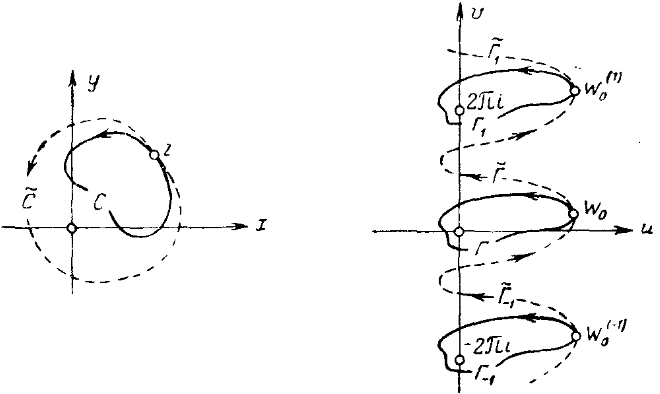
\includegraphics[width=.8\linewidth]{mal-14.png}
	% \caption{дія логарифму на різні криві}
\end{figure}

Звідси випливає, що у довільній області $D$ яка не містить замкнутих кривих які обходять точку $z = 0$ можна виділити \textit{нескінченну множину неперервних і однозначних гілок} багатозначної функції $w = \Ln z$, значення яких у кожній фіксованій точці відрізняються на доданок $2 k \pi i$. \\

Кожна така гілка $\ln z$ буде реалізувати взаємно-однозначне відображення області $D$ і, відповідно, за теоремою про прохідну оберненої функції буде мати \textit{похідну}
\begin{equation}
	\label{eq:3.3.16}
	(\ln z)' = \dfrac{1}{(e^w)'} = \dfrac{1}{e^w} = \dfrac 1z.
\end{equation}

Зауважимо, що похідна \textit{одна} для усіх гілок. \\

Таким чином, всі гілки $\Ln z$ будуть \textit{аналітичними} функціями. \\

Якщо ж область $D$ містить хоча б одну замкнуту криву що охоплює точку $z = 0$, то у такій області гілки функції $\Ln z$ розрізнити \textit{неможливо}. \\

Точка $z = 0$ у якій немовби з'єднуються всі гілки функції $\Ln z$ називається точкою \textit{гілкування}.

\subsection{Тригонометричні та гіперболічні функції}

\subsubsection{Тригонометричні функції}

У комплексній області просто виражаються через експоненту. \\

Для дійсної змінної $x$ формула Ейлера дає
\begin{equation}
	\label{eq:3.4.1}
	e^{i x} = \cos x + i \sin x, \quad e^{-i x} = \cos x - i \sin x,
\end{equation}
звідки
\begin{equation}
	\label{eq:3.4.2}
	\sin x = \dfrac{e^{i x} - e^{-i x}}{2i}; \quad \cos x = \dfrac{e^{i x} + e^{-i x}}{2}.
\end{equation}

Використаємо це як визначення, тобто нехай для довільного комплексного $z$:
\begin{equation}
	\label{eq:3.4.3}
	\sin z = \dfrac{e^{i z} - e^{-i z}}{2i}; \quad \cos z = \dfrac{e^{i z} + e^{-i z}}{2}.
\end{equation}

Таким чином визначені функції для дійсних $z = x$ збігаються зі звичайними синусом і косинусом. \\

Також, обидві визначені функції всюди аналітичні, причому виконуються звичайні формули диференціювання:
\begin{equation}
	\label{eq:3.4.4}
	(\sin z)' = \cos z; \quad (\cos z)' = - \sin z.
\end{equation}

Обидві функції періодичні з дійсним періодом $2 \pi$. \\

$\sin z$ -- непарна функція, $\cos z$ -- парна. \\

Виконуються звичайні тригонометричні рівності:
\begin{equation}
	\label{eq:3.4.5}
	\sin^2 z + \cos^2 z = 1, \quad \sin 2z = 2 \sin z \cos z, \quad \ldots
\end{equation}

Дослідимо відображення яке реалізує перша з цих функцій. Покладаючи
\begin{equation}
	\label{eq:3.4.6}
	iz = z_1, \quad e^{z_1} = z_2, \quad z_3 = -i z_2 = \dfrac{e^{i z}}{i},
\end{equation}
отримаємо
\begin{equation}
	\label{eq:3.4.7}
	w = \dfrac 12 \left( z_3 + \dfrac{1}{z_3} \right) = \sin z.
\end{equation}

Таким чином, наше відображення можна розглядати як композицію вже досліджених. \\

Знайдемо перш за все умови його однолистості: нехай $D$ при відображеннях \eqref{eq:3.4.6} переходить послідовно в $D_1$, $D_2$ і $D_3$. \\

Перше і третє із відображень \eqref{eq:3.4.6} однолисті всюди, а для однолистості другого необхідно і достатньо аби $D_1$ не містила жодної пари точок $z_1'$ і $z_1''$ пов'язаних співвідношенням $z_1' - z_1'' = 2 k \pi i$, де $k$ -- ціле число. \\

Для однолистості відображення \eqref{eq:3.4.7} необхідно і достатньо аби область $D_3$ не містила жодної пари точок $z_3'$ і $z_3''$ пов'язаних співвідношенням $z_3' \cdot z_3'' = 1$.

Переходячи за допомогою формул \eqref{eq:3.4.6} до площини $z$ отримаємо, що для однолистості відображення $w = \sin z$ в області $D$ необхідно і достатньо, аби $D$ не містила жодної пари точок $z'$ і $z''$ пов'язаних, по-перше
\begin{equation}
	\label{eq:3.4.8}
	z' - z'' = 2 k \pi \quad (k \ne 0\text{ -- ціле}),
\end{equation}
і, по-друге, співвідношенням $e^{i(z' + z'') = -1}$, або, що те саме,
\begin{equation}
	\label{eq:3.4.9}
	z' + z'' = (2k + 1) \cdot \pi \quad (k\text{ -- ціле}),
\end{equation}

Цим умовам задовольняє, наприклад, півсмуга $- \pi < x < \pi$, $y > 0$:
\begin{figure}[H]
	\centering
	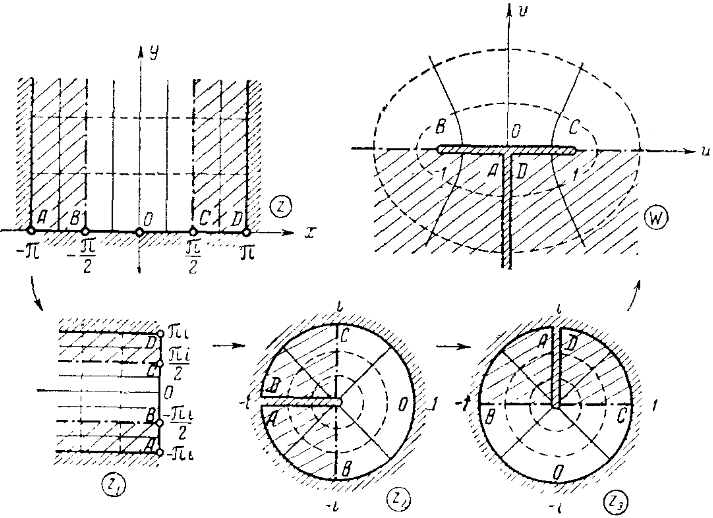
\includegraphics[width=.8\linewidth]{mal-15.png}
	%\caption{послідовні відображення півсмуги $- \pi < x < \pi$, $y > 0$}
\end{figure}

Сім'ї променів $x = x_0$ і відрізків $y = y_0$ переходять в сім'ї гіпербол та еліпсів відповідно, зі спільними фокусами. \\

При цьому вдвічі вужча півсмуга $- \dfrac{\pi}{2} < x < \dfrac{\pi}{2}$, $y > 0$ переходить у верхню півплощину. \\

Як бачимо, $\sin z$ в комплексній площині не є обмеженим, наприклад на променях $x = \pm \pi/2$, $y > 0$ він набуває дійсних значень за модулем більших за одиницю, і взагалі як завгодно великих. \\

Помітимо також, що у (замкнутій) півсмузі $- \pi \le x \le \pi$, $y \ge 0$ функція $\sin z$ набуває значення 0 лише у точках $z = 0$ і $z = \pm \pi$. \\

Враховуючи непарність і періодичність цієї функції, можна зробити висновок що вона обертається на нуль лише на дійсній вісі у точках $z = k \pi$. \\

Для повноти приводимо \textit{поверхню модуля}, або ``рельєф'' функції $\sin z$, тобто поверхню у просторі $(x,y,u)$ з рівнянням $u=|\sin z|$:

\begin{figure}[H]
	\centering
	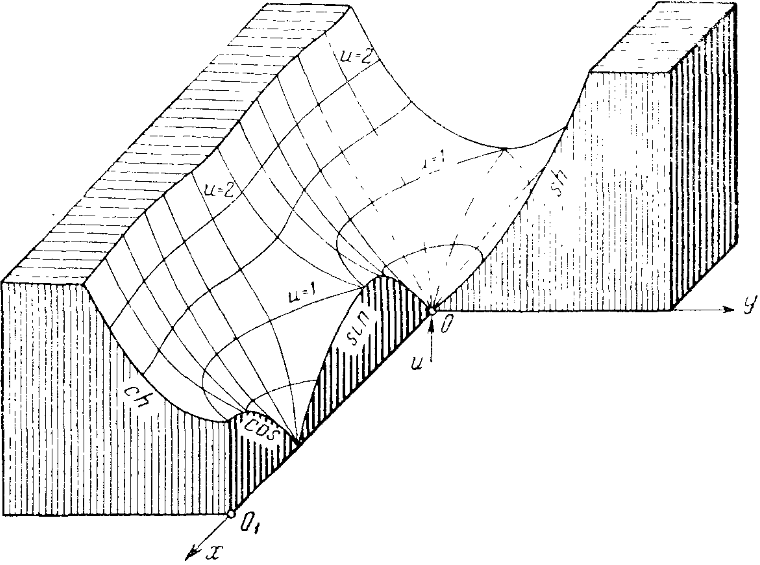
\includegraphics[width=.8\linewidth]{mal-16.png}
\end{figure}

Ця поверхня періодична з дійсним періодом $\pi$. \\

На ній нанесені дві системи ліній -- це лінії рівня $|\sin z|$ і $\arg \sin z$. \\

Зріз поверхні вертикальною площиною, що проходить через вісь $Ox$ дає графік функції $|\sin x|$. \\

По мірі віддалення від цієї осі поверхня згладжується, а аплікати ($u$-координати) її точок швидко зростають. \\

За формою поверхня наближається до циліндра $u = e^{|y|} / 2$. \\

Відображення яке реалізує функція $\cos z$, у силу співвідношення
\begin{equation}
	\label{eq:3.4.10}
	\cos z = \sin \left( z + \dfrac \pi 2 \right)
\end{equation}
відрізняється від розглянутого виключно зсувом. \\

Функції $\tan z$ і $\cot z$ визначаються формулами
\begin{equation}
	\label{eq:3.4.11}
	\tan z = \dfrac{\sin z}{\cos z} = - i \dfrac{e^{i z} - e^{-i z}}{e^{i z} + e^{-i z}}; \quad \cot z = \dfrac{\cos z}{\sin z} = i \dfrac{e^{i z} + e^{-i z}}{e^{i z} - e^{-i z}}.
\end{equation}

Функція $\tan z$ аналітична всюди за виключенням точок де $\cos z$ обертається на нуль, тобто всюди окрім точок $z_k = \pi/2 + k \pi$, адже при наближенні до цих точок $\tan z$ необмежено зростає. \\

Те ж саме можна сказати про функцію $\cot z$ і точки $z_k = k \pi$. \\

З формул \eqref{eq:3.4.11} випливає, що ці функції періодичні з періодом $\pi$. Справді,
\begin{equation}
	\label{eq:3.4.12}
	\tan (z + \pi) = -i \dfrac{e^{i(z + \pi} - e^{-i(z + \pi)}}{e^{i(z + \pi} + e^{-i(z + \pi)}} = -i \dfrac{-e^{i z} + e^{-i z}}{-e^{i z} - e^{-i z}} = \tan z.
\end{equation}

Відображення яке реалізує функція $w = \tan z$ ми розглянемо пізніше. \\

Тут ми наведедемо лише рельєф тангенсу, тобто поверхню $u = |\tan z|$:

\begin{figure}[H]
	\centering
	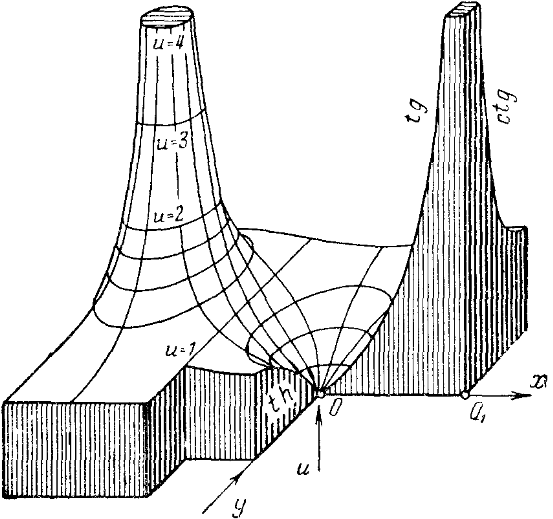
\includegraphics[width=.6\linewidth]{mal-17.png}
\end{figure}

Ця поверхня періодична з дійсним періодом $\pi/2$. \\

Вона має яскраво виражені піки над точками $z = \pi / 2 + k \pi$,$k = 0, \pm 1, \pm 2, \ldots$.\\

Її зріз вертикальною площиною, що проходить через вісь $Ox$, дає графік $|\tan x|$. \\

По мірі віддалення від цієї вісі поверхня стає все більш плоською і наближається до площини $u = 1$. \\

На поверхні нанесені лінії рівня $|\tan z|$ і $\arg \tan z$.\\

\subsubsection{Гіперболічні функції}

Гіперболічні функції у комплексній області визначається рівностями
\begin{align}
	\label{eq:3.4.13}
	\sinh z &= \dfrac{e^z - e^{-z}}{2}, \\
	\label{eq:3.4.14} 
	\cosh z &= \dfrac{e^z + e^{-z}}{2}, \\
	\label{eq:3.4.15}
	\tanh z &= \dfrac{\sinh z}{\cosh z} = \dfrac{e^z - e^{-z}}{e^z + e^{-z}}, \\
	\label{eq:3.4.16}
	\coth z &= \dfrac{\cosh z}{\sinh z} = \dfrac{e^z + e^{-z}}{e^z - e^{-z}}.
\end{align}

Вони цілком просто виражаються через тригонометричні функції:
\begin{align}
	\label{eq:3.4.17}
	\sinh z &= - i \sin i z, \\
	\label{eq:3.4.18}
	\cosh z &= \cos i z, \\
	\label{eq:3.4.19}
	\tanh z &= -i \tan i z, \\
	\label{eq:3.4.20}
	\coth z &= i \cot i z,
\end{align}
і тому несуттєво від них відрізняються. \\

\subsubsection{Обернені тригонометричні та гіперболічні функції}

Тригонометричні та гіперболічні функції виражаються через експоненту, тому обернені тригонометричні і обернені гіперболічні функції виражаються через логарифми. \\

Отримаємо такий вираз для $w = \arccos z$: за визначенням
\begin{equation}
	\label{eq:3.4.21}
	z = \cos w = \dfrac{e^{iw} + e^{-iw}}{2},
\end{equation}
звідки 
\begin{equation}
	\label{eq:3.4.22}
	e^{2 i w} - 2 z e^{i w} + 1 = 0.
\end{equation}

Розв'язуючи це квадратне відносно $e^{i w}$ рівняння, знаходимо
\begin{equation}
	\label{eq:3.4.23}
	e^{i w} = z + \sqrt{z^2 - 1}
\end{equation}
і
\begin{equation}
	\label{eq:3.4.24}
	w = \arccos z = -i \ln (z + \sqrt{z^2 - 1})
\end{equation}
(знаки $\pm$ у формулі коренів квадратного рівняння можна опустити якщо розуміти корінь як двозначну функцію). \\

У силу співвідношення
\begin{equation}
	\label{eq:3.4.25}
	(z + \sqrt{z^2 - 1}) \cdot (z - \sqrt{z^2 - 1}) = 1
\end{equation}
зміна знаку перед коренем зводиться до зміни знаку перед логарифмом, тому знак ''$-$'' в останній формулі також можна не писати:
\begin{equation}
	\label{eq:3.4.26}
	w = \arccos z = i \ln (z + \sqrt{z^2 - 1})
\end{equation}

Аналогічні формули можна отримати й для інших функцій:
\begin{align}
	\label{eq:3.4.27}
	\arcsin z &= \dfrac{\pi}{2} - \arccos z = \dfrac{\pi}{2} - i \ln (z + \sqrt{z^2 - 1}), \\
	\label{eq:3.4.28}
	\arctan z &= \dfrac{\pi}{2} - \arctan z = \dfrac{1}{2 i} \cdot \ln \left( \dfrac{1 + i z}{1 - i z} \right), \\
	\label{eq:3.4.29}
	\arcsinh z &= \ln (z + \sqrt{z^2 + 1}), \\
	\label{eq:3.4.30}
	\arccosh z &= \ln (z + \sqrt{z^2 - 1}), \\
	\label{eq:3.4.31}
	\arctanh z &= \dfrac 12 \cdot \ln \left( \dfrac{1 + z}{1 - z} \right), \\
	\label{eq:3.4.32}
	\arccoth z &= \dfrac 12 \cdot \ln \left( \dfrac{z + 1}{z - 1} \right).
\end{align}

Всі ці функції багатозначні, адже $\ln$ у правій частині формул \eqref{eq:3.4.26}-\eqref{eq:3.4.32} може позначати довільне значення логарифму. \\

Способи виділення їх однозначних гілок аналогічні розглянутим вище. \\

Всі такі гілки будуть аналітичними функціями.

\subsection{Загальна степенева функція $w = z^a$}

Визначається співвідношенням
\begin{equation}
	\label{eq:3.5.1}
	z^a = e^{a \Ln z},
\end{equation}
де $a = \alpha + i \beta$. \\

Покладаючи $z = r \cdot e^{i \phi}$, отримаємо
\begin{equation}
	\label{eq:3.5.2}
	\Ln z = \ln r + i (\phi + 2 k \pi)
\end{equation}
 і, як наслідок,
\begin{equation}
	\label{eq:3.5.3}
	z^a = e^{\alpha \ln r - \beta (\phi + 2 k \pi)} \cdot e^{i (\alpha (\phi + 2 k \pi) + \beta \ln r)},
\end{equation}
де $k$ -- ціле число. \\

Звідси видно, що при $\beta \ne 0$ функція $z^a$ завжди має нескінченно багато значень які лежать (при фіксованих $z$ і $a$) на колах $|w| = \rho_k$ з радіусами
\begin{equation}
	\label{eq:3.5.4}
	\rho_k = e^{\alpha \ln r - \beta \phi} \cdot e^{-2 k \pi \beta}
\end{equation}
які утворюють геометричну нескінченну в обидві сторони прогресію зі знаменником $e^{-2 \pi \beta}$. \\

Аргументи цих значень
\begin{equation}
	\label{eq:3.5.5}
	\theta_k = \alpha \phi + \beta \ln r + 2 k \pi \alpha
\end{equation}
утворюють також нескінченну в обидві сторони арифметичну прогресію з різницею $2 \pi \alpha$. \\

При $\beta = 0$, тобто при дійсних $a$, значення $z^a$ розташовані на колі $|w| = e^{a \ln r} = r^a$, і їх аргументи є
\begin{equation}
	\label{eq:3.5.6}
	\theta_k = a \phi + 2 k \pi a.
\end{equation}

Якщо $a = p / q$ -- раціональне число, то всі значення $\theta_k$ будуть відрізнятися від $q$ із цих значень на ціле кратне $2 \pi$. \\

Як наслідок, у цьому випадку функція $w = z^a$ скінченно-значна і збігається із функцією $\sqrt[q]{z^p}$:
\begin{equation}
	\label{eq:3.5.7}
	z^{p / q} = \sqrt[q]{z^p}.
\end{equation}

Якщо ж $a$ -- ірраціональне дійсне число, то серед значень $\theta_k$ у формулі \eqref{eq:3.5.6} немає таких, які відрізняються на ціле кратне $2 \pi$ і, як наслідок, функція $z^a = e^{a \Ln z}$ нескінченнозначна. \\

Багатозначність загальної степеневої функції, як і тих елементарних функцій, які ми розглядали вище, обумовлена багатозначністю аргументу. \\

Способи виділення її однозначних гілок попереднє, точкою гілкування є $z = 0$. \\

Наряду із загальною степеневою функцією \eqref{eq:3.5.1} можна розглядати загальну експоненту
\begin{equation}
	\label{eq:3.5.8}
	a^z = e^{z \Ln a} = e^{z \ln |a|} \cdot e^{z i \Arg a}.
\end{equation}

На відміну від функції \eqref{eq:3.5.1} функція \eqref{eq:3.5.8} являє собою сукупність окремих, не зв'язаних між собою однозначних функцій, які відрізняються множниками $e^{2 k \pi i z}$, де $k$ -- ціле число.

% \flushright{\copyright \, М. А. Лаврентьев, Б. В. Шабат, 1972 \\ Українською переклав Н. М. Скибицький, 2018}

% \end{document}